% Competing-analyses version of the evidence-to-policy diagram: one piece of
% research feeds three rival policy analyses, and each policy maker picks the
% one that suits them. Redrawn in the style of evidence-to-policy.tex from the
% dissertation figure (dissertation-manuscript/dissertation.tex, label
% med_cred). Built by ./build.sh as the "competing" variant.

\documentclass[border=10pt,tikz]{standalone}
\usepackage{tikz}
\usetikzlibrary{positioning,shapes.geometric,decorations.pathreplacing,calc}
\pdftrailerid{}

\begin{document}
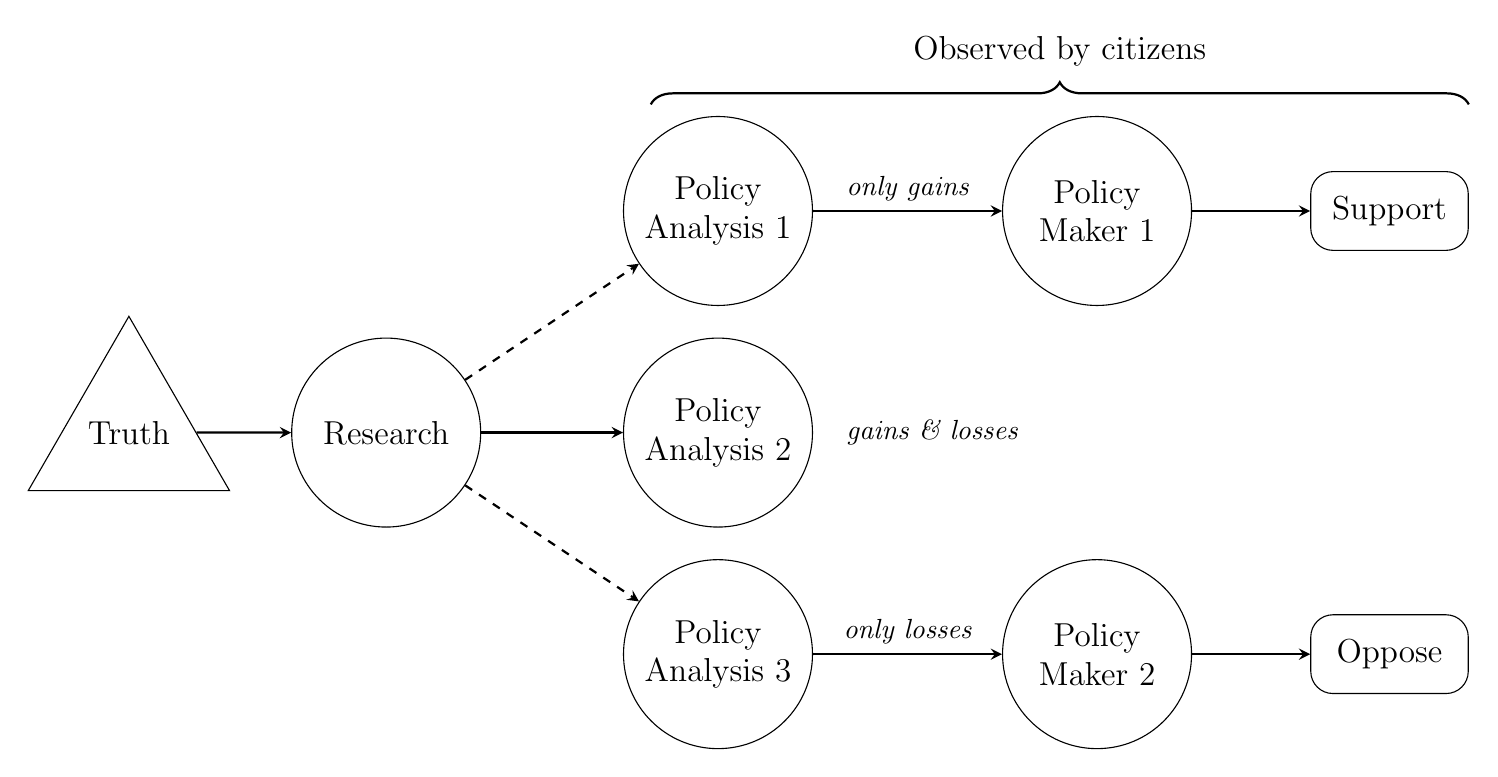
\begin{tikzpicture}[
  every node/.style={font=\large},
  bigcirc/.style={circle, draw, minimum size=2.4cm, align=center, inner sep=2pt},
  tri/.style={regular polygon, regular polygon sides=3, draw,
              minimum size=2.5cm, align=center, inner sep=0pt},
  rrect/.style={rectangle, rounded corners=8pt, draw, minimum width=2cm,
                minimum height=1cm, align=center},
  arr/.style={-stealth, thick},
  darr/.style={-stealth, thick, dashed},
  note/.style={font=\normalsize\itshape}
]

\node[tri]                                  (T)   {Truth};
\node[bigcirc, right=1.2cm of T]            (R)   {Research};
\node[bigcirc, right=1.8cm of R]            (PA2) {Policy\\Analysis 2};
\node[bigcirc, above=0.4cm of PA2]          (PA1) {Policy\\Analysis 1};
\node[bigcirc, below=0.4cm of PA2]          (PA3) {Policy\\Analysis 3};
\node[bigcirc, right=2.4cm of PA1]          (PM1) {Policy\\Maker 1};
\node[bigcirc, right=2.4cm of PA3]          (PM2) {Policy\\Maker 2};
\node[rrect,   right=1.5cm of PM1]          (S)   {Support};
\node[rrect,   right=1.5cm of PM2]          (O)   {Oppose};

\draw[arr]  (T)   -- (R);
\draw[darr] (R)   -- (PA1);
\draw[arr]  (R)   -- (PA2);
\draw[darr] (R)   -- (PA3);
\draw[arr]  (PA1) -- node[note, above] {only gains} (PM1);
\draw[arr]  (PA3) -- node[note, above] {only losses} (PM2);
\node[note, right=0.3cm of PA2] {gains \& losses};
\draw[arr]  (PM1) -- (S);
\draw[arr]  (PM2) -- (O);

% What citizens see: the rival analyses and what each policy maker does.
\coordinate (bl) at ($(PA1.north west)+(0,0.5)$);
\draw[decorate, decoration={brace, amplitude=8pt}, thick]
  (bl) -- (bl -| S.east) node[midway, above=10pt] {Observed by citizens};

\end{tikzpicture}
\end{document}
